% vim: ts=8 sts=8 sw=4 et tw=75
\chapter{小型语言}
\label{chap:little_languages}
\marginpar{131}

人们经常使用 awk 开发 ``小型语言'' 的翻译器 (``小型语言'' 指的特定于
某些应用领域的专用编程语言), 
开发翻译器的原因主要有三点. 首先, 它可以帮助你了解语言处理程序的工作流程.
本章的第一个例子是一个汇编程序, 虽然只有 20 来行, 但已经包含了汇编过程
的核心要素, 为了执行汇编程序, 我们还要开发一个解释器程序. 汇编程序与
解释器反映了早期阶段 汇编语言与机器架构的关系. 其他例子还包括一个
后缀计算器, awk 子集的递归下降分析器.

第二个原因是在实际工作中, 为了实现一个专用的编程语言, 通常需要投入大
量的精力与财力, 不过在这之前, 我们有必要测试一下新语言的语法和语义. 
作为示例, 本章讨论了一个画图语言和一个参数设置语言, 后者用于设置排序命令
的参数.

最后一点是希望编程语言能够在实际的工作发挥作用, 就比如说本章所开发的
计算器.

语言处理程序围绕下面这个模型构造而成:
\begin{center}
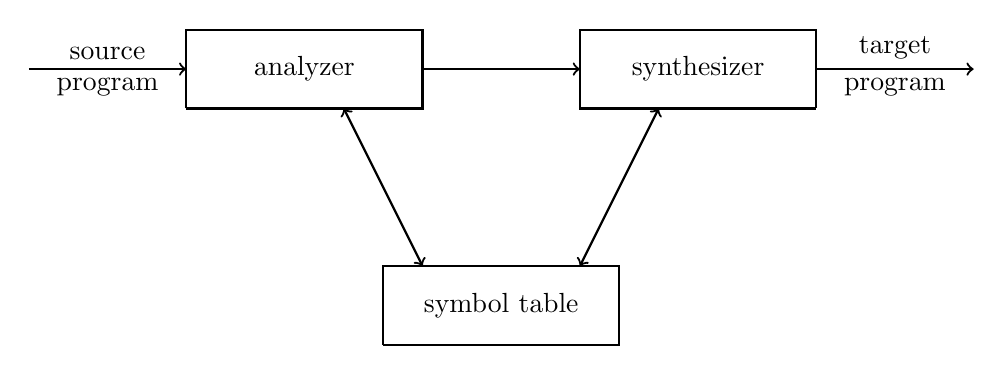
\begin{tikzpicture}
    \draw[thick]
        (-1.5, 0) -- (-1.5, 1.0) -- (1.5, 1.0) -- (1.5, 0) -- (-1.5, 0);
    \draw[thick]
        (-4.0, 3.0) -- (-4.0, 4.0) -- (-1.0, 4.0) -- (-1.0, 3.0) -- (-4.0,
        3.0);
    \draw[thick]
        (4.0, 3.0) -- (4.0, 4.0) -- (1.0, 4.0) -- (1.0, 3.0) -- (4.0, 3.0);
    
    \draw[thick,->]
        (-6.0, 3.5) -- (-4.0, 3.5);
    \draw[thick,->]
        (-1.0, 3.5) -- (1.0, 3.5);
    \draw[thick,->]
        (4.0, 3.5) -- (6.0, 3.5);
    \draw[thick,<->]
        (-2.0, 3.0) -- (-1.0, 1.0);
    \draw[thick,<->]
        (2.0, 3.0) -- (1.0, 1.0);

    \node[above] at (-5.0, 3.5) {source};
    \node[below] at (-5.0, 3.5) {program};
    \node at (-2.5, 3.5) {analyzer};
    \node at (2.5, 3.5) {synthesizer};
    \node[above] at (5.0, 3.5) {target};
    \node[below] at (5.0, 3.5) {program};
    \node at (0, 0.5) {symbol table};
\end{tikzpicture}
\end{center}

分析器 (analyzer) 系语言处理程序的前端, 它负责读取源程序 (source program)
并将其切分成 一个个词法单元, 词法
单元包括运算符, 操作数等. 分析器对源程序进行语法检查, 如果源程序含有语法
错误, 它就会打印一条错误消息. 最后, 分析器把源程序转换成某种中间形式,
并传递给后端 (合成器), 合成器 (synthesizer) 再根据中间形式生成目标程序
(target program). 合成器在生成
目标程序的过程中需要和符号表 (symbol table) 通信, 而符号表中的内容由分析
器收集而来.
虽然我们把语言的处理过程描述成多个界限分明的不同步骤, 但实际上, 这些界限
通常很模糊, 而且有些步骤有可能被合并成一个.
\marginpar{132}
